\chapter{Asking a 27-Year-Old How to Make \$300 Million}

These notes follow a School of Hard Knocks interview with Zane, curated by LazyingArt LLC with Video2Book. The material is not a blackboard lecture in the literal sense; its mathematics is the arithmetic of scale, ratios, thresholds, and operating mechanisms. We therefore read the interview as a sequence of claims: what was said, what mechanism was proposed, and where the numbers illuminate the judgment.

\section{The Opening Number}

The interview begins with the number before it gives us the full story. The host asks whether Zane is the chief executive of one of the largest solar companies in the country, then asks for the largest amount of money the business has made in a single year. Zane says the business did \(\$149\mathrm{M}\) last year and should roughly double that this year.

The arithmetic is simple, but it is the first anchor of the chapter:
\begin{equation}
149\,\mathrm{M}\times 2 = 298\,\mathrm{M}\approx 300\,\mathrm{M}.
\end{equation}
This should be read as an interview claim, not as audited financial reporting. Its function in the conversation is to establish scale. We are not yet asking whether the number is enough to define durable wealth. We are first asking what sort of business machinery could plausibly move from one large number to the next.

The operating context follows a minute later. Zane describes the company as a large residential solar installer in Miami, with more than \(600\) W2 employees and more than \(3000\) sales representatives selling through it:
\begin{equation}
\text{W2 employees}>600,\qquad \text{sales reps}>3000.
\end{equation}
That contrast matters. The company is not presented merely as a personal brand or a one-person sales operation. The transcript frames it as an organization with employees, distributed sales capacity, and repeatable installation activity.

\section{From Salesperson to Owner}

The host then pulls the story backward. Zane says he grew up lower class, with first-generation immigrant parents who did not speak English. At eighteen he decided to go all in on sales, then moved into solar sales. The sequence he gives is direct:
\begin{equation}
\text{salesperson}\longrightarrow \text{sales leader}\longrightarrow \text{business owner}.
\end{equation}

The mechanism here is not capital, inheritance, or a technical invention. The first mechanism is sales skill. In the language of this book, sales is the original conversion function: it turns contact with a customer into revenue, and it turns personal effort into a path toward ownership. Zane's account places that skill before later discussions of systems, networks, and reinvestment.

This is also where the interview sets up one of its recurring distinctions. A person can make money by selling. A company can become valuable only when the selling is embedded in a larger structure. The rest of the interview asks how that structure appears.

\section{Seven, Eight, and Nine Figures}

The first major business question is about scale. The host asks what allowed the company to move from seven figures to eight figures and then toward nine figures. Zane answers with a ladder.

\begin{align}
7\text{-figure scale} &\Rightarrow \text{idea}+\text{sales}+\text{marketing},\\
8\text{-figure scale} &\Rightarrow \text{team},\\
9\text{-figure scale} &\Rightarrow \text{product}+\text{marketing}+\text{sales}+\text{team}+\text{systems}.
\end{align}

In his formulation, the first level can still depend heavily on the founder's personal energy and sales ability. The next level requires people. But the nine-figure level requires something more impersonal: standard operating procedures, or SOPs.

\begin{figure}
\centering
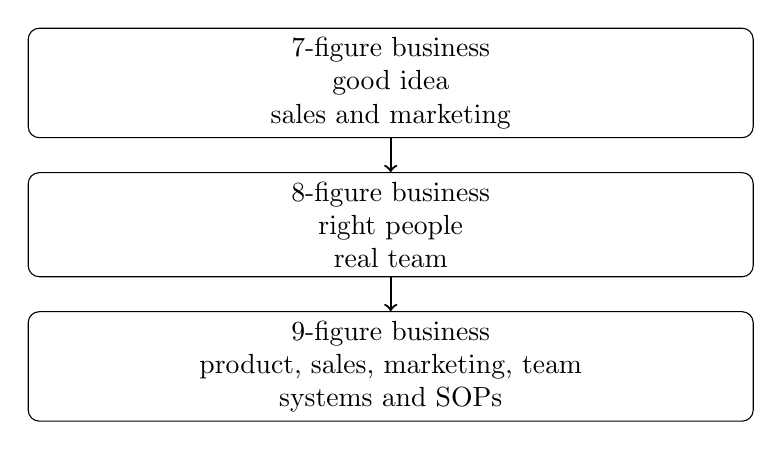
\begin{tikzpicture}[
  node/.style={draw, rounded corners, align=center, text width=.74\linewidth, minimum height=1.0cm},
  arrow/.style={->, thick}
]
\node[node] (a) at (0,0) {\(7\)-figure business\\good idea\\sales and marketing};
\node[node] (b) at (0,-1.8) {\(8\)-figure business\\right people\\real team};
\node[node] (c) at (0,-3.6) {\(9\)-figure business\\product, sales, marketing, team\\systems and SOPs};
\draw[arrow] (a) -- (b);
\draw[arrow] (b) -- (c);
\end{tikzpicture}
\caption{Zane's scaling ladder as a transcript-backed operating model.}
\end{figure}

\subsection{Question \& Answer}

\paragraph{Question.}
Why does the chief executive become the bottleneck as the business grows?

\paragraph{Answer.}
Because undocumented work stays trapped inside a person. Zane's example is deliberately exaggerated: he says there is a standard operating procedure for everything, even ordinary functions such as making coffee. The point is not the coffee. The point is transferability. If a function is documented, then another person can perform it when the original operator is absent.

We can write the mechanism as a small update rule:
\begin{equation}
\text{undocumented function}
\longrightarrow
\text{documented function}
\longrightarrow
\text{transferable function}
\longrightarrow
\text{lower founder dependence}.
\end{equation}

That is the central business claim of the scaling section. At eight figures, people may still rely on the CEO. At nine figures, Zane says, they rely on the machine and the system. The most vivid version of the claim is that even if the CEO disappears, the system should continue to operate.

\begin{figure}
\centering
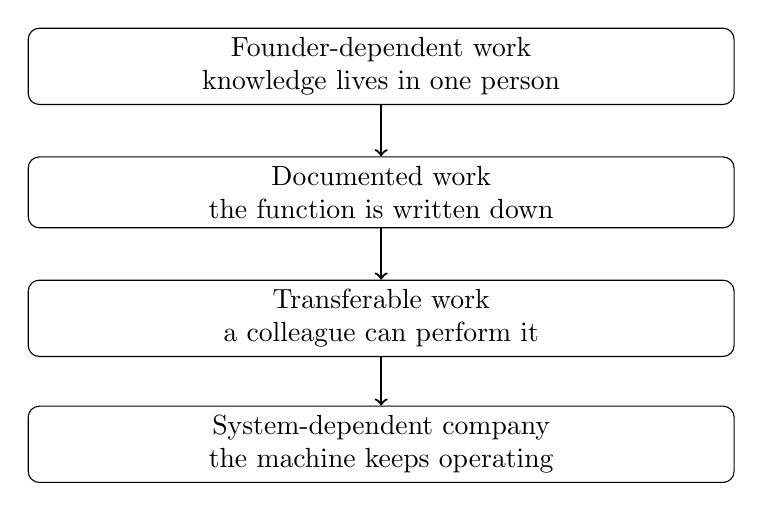
\begin{tikzpicture}[
  node/.style={draw, rounded corners, align=center, text width=.72\linewidth, minimum height=.9cm},
  arrow/.style={->, thick}
]
\node[node] (a) at (0,0) {Founder-dependent work\\knowledge lives in one person};
\node[node] (b) at (0,-1.6) {Documented work\\the function is written down};
\node[node] (c) at (0,-3.2) {Transferable work\\a colleague can perform it};
\node[node] (d) at (0,-4.8) {System-dependent company\\the machine keeps operating};
\draw[arrow] (a) -- (b);
\draw[arrow] (b) -- (c);
\draw[arrow] (c) -- (d);
\end{tikzpicture}
\caption{The founder-dependence reduction described in the interview.}
\end{figure}

\section{Moving Closer to the Money}

The next pivot is personal rather than organizational. The host asks about escaping poverty. Zane's answer is blunt: in his view, a person cannot get rich while remaining inside a poor environment. We should not turn that into a universal theorem. It is an interview claim, based on his experience, about motivation, access, and proximity.

The mechanism he gives has three parts. First, build skill while trapped. Second, save enough money to move. Third, relocate toward a denser economy where money, customers, operators, and ambition are more visible.

The transcript gives a numerical contrast. In one environment, everyone around you may be making about \(\$40{,}000\) per year. In another, Zane imagines a city where, within a \(30\)-mile radius, there may be \(14\) billionaires and tens of thousands of multimillionaires:
\begin{equation}
r=30\ \mathrm{miles},\qquad
N_{\mathrm{billionaires}}\approx 14,\qquad
N_{\mathrm{multimillionaires}}=\text{tens of thousands}.
\end{equation}
Again, these are not verified demographics in the chapter. They are Zane's way of quantifying proximity to opportunity.

The causal picture is qualitative:
\begin{equation}
\text{skill}+\text{relocation}+\text{opportunity density}
\Rightarrow
\text{higher chance of useful contact and commerce}.
\end{equation}
That implication should not be overstated. It does not say that location guarantees success. It says that the environment changes the rate at which one encounters money, standards, and possible commercial relationships.

\section{Networks Require Value Before Access}

After the sponsor interruption, the interview returns to relationships. The host asks how Zane has leveraged relationships and what advice he would give someone trying to build a network. Zane answers with a hard premise: successful people focus on what adds value to their lives. If one brings no value, one should not expect value in return.

This is the second major bottleneck in the interview. Earlier, the bottleneck was founder dependence. Here the bottleneck is social value. Access to a room is not the same thing as a relationship inside that room.

\subsection{Question \& Answer}

\paragraph{Question.}
Why does meeting a billionaire not automatically create a useful relationship?

\paragraph{Answer.}
Because contact is not the same as earned access. Zane gives the example of running into Elon Musk in the street. The meeting might be exciting. It might even create content. But that does not imply a phone number, a returned call, or a durable channel of trust.

A useful relationship requires some combination of value, relevance, and earned respect:
\begin{equation}
\text{durable relationship}
\neq
\text{accidental contact}.
\end{equation}
A more useful model is
\begin{equation}
\text{durable relationship}
\Rightarrow
\text{access}+\text{value}+\text{trust}+\text{reciprocity}.
\end{equation}

Zane then adds a negative version of the same principle. It is not only about whom one spends time with; it is also about whom one avoids. A person can be excluded from better rooms because the people around him bring down the group. The practical mechanism is reputational: companions can either amplify or discount one's perceived value.

\section{Spend Money, But Put It to Work}

The host next asks for the best financial advice Zane ever received. Zane answers with a reversal: spend your money. This sounds, at first, like it contradicts the earlier advice to save enough to move. The contradiction disappears once we separate stages and uses of capital.

At the escape stage, money is saved for skill and relocation. At the operating stage, excess cash should not sit idle after expenses, operating costs, and payroll are covered. Zane frames a full bank account as a vehicle with no fuel if the money is not working.

Let \(C\) denote cash in the business after required obligations. Let \(O\) denote operating requirements: expenses, payroll, and near-term needs. The relevant excess is
\begin{equation}
C_{\mathrm{excess}} = C - O.
\end{equation}
Zane's advice is not that every dollar should be consumed. It is that excess capital should be deployed:
\begin{equation}
C_{\mathrm{excess}}
\longrightarrow
\text{business capacity, skill, people, systems, or assets}.
\end{equation}

\paragraph{Worked example.}
The transcript's logic can be written as a simple decision rule.

\begin{enumerate}
\item Cover required operating costs and payroll.
\item Identify excess cash:
\[
C_{\mathrm{excess}}=C-O.
\]
\item If \(C_{\mathrm{excess}}>0\), ask whether the cash is protecting a real risk or merely creating comfort.
\item If it is merely creating comfort, deploy it into the business or into personal capability.
\item The goal is to raise the value of the main asset rather than admire idle cash.
\end{enumerate}

This is not universal financial advice. It is Zane's operating doctrine for a growth business whose owner believes the main net-worth engine is the company itself. The important distinction is between consumption and deployment.

\section{Conviction, Riches, and Wealth}

The sales section returns to the first mechanism of the interview. The host asks how Zane has sold at high volume across his career. Zane rejects a purely tactical view of selling. Scripts, objection handling, and role plays matter, but he says the dominant variable is conviction in the product.

His rough weighting is:
\begin{equation}
\text{sales effectiveness}
\approx
10\%\,(\text{tactics})+90\%\,(\text{conviction}).
\end{equation}
This is rhetorical, not statistical. But it captures the lesson: buyers sense enthusiasm, belief, and hesitation. A trained salesperson who does not believe in the product may lose to a less trained salesperson who does.

The interview then shifts from selling to the difference between rich and wealthy. Zane defines ``rich'' as earning roughly \(\$4\mathrm{M}\) to \(\$10\mathrm{M}\) per year, while ``wealthy'' means, in his framing, billionaire-level deployed assets:
\begin{align}
\text{rich} &\sim \$4\mathrm{M}\text{--}\$10\mathrm{M}\ \text{per year},\\
\text{wealthy} &\sim \$1\mathrm{B}\ \text{in deployed assets}.
\end{align}

The distinction is not only size. It is deployment. Wealth, in this answer, means money working in businesses, private equity, stocks, real estate, and other assets. Idle cash does not have the same status.

Zane illustrates the point with a yacht example. If a person has \(\$100\mathrm{M}\) and buys or operates a luxury asset costing \(\$12\mathrm{M}\) per year to run, the annual cost is a large fraction of net worth:
\begin{equation}
\frac{\$12\mathrm{M}}{\$100\mathrm{M}}
=
0.12
=
12\%.
\end{equation}
At \(\$1\mathrm{B}\), a \(\$50\mathrm{M}\) purchase is still significant, but the ratio is different:
\begin{equation}
\frac{\$50\mathrm{M}}{\$1\mathrm{B}}
=
0.05
=
5\%.
\end{equation}
The lesson is not about yachts in particular. It is about scale changing the meaning of spending. A toy that is survivable at one balance-sheet size can be destructive at another.

\section{Summary}

The interview begins with a revenue claim and ends with a compressed rule: learn sales and do not quit. Between those points, Zane gives a sequence of mechanisms. Sales creates the first opening. Team extends the business beyond the founder. SOPs turn work into transferable machinery. Environment changes the density of opportunity. Relationships require value before access. Money should be deployed rather than hoarded once the operating base is protected. Wealth, in his strict framing, is not merely high income but capital working through durable assets.

The chapter's numbers should stay attached to their source. The \(\$149\mathrm{M}\), \(\$300\mathrm{M}\), \(600\)-employee, \(3000\)-rep, \(10/90\), and yacht-cost examples are all interview claims or illustrative calculations. Their value is not that they form a universal law. Their value is that they reveal the commercial logic of one operator who describes the passage from personal selling to institutional scale.